% Ujian CPMK-2: Reasoning — Fuzzy System Pemilihan Konsentrasi Mahasiswa
% Format IEEE Conference, 2 kolom
\documentclass[conference]{IEEEtran}
\usepackage[utf8]{inputenc}
\usepackage[T1]{fontenc}
\usepackage{amsmath,amssymb}
\usepackage{booktabs}
\usepackage{enumitem}
\usepackage{array}
\usepackage{multirow}
\usepackage{tikz}
\usetikzlibrary{positioning,arrows.meta,shapes.geometric}
\usepackage{hyperref}
\hypersetup{colorlinks=true,linkcolor=blue,citecolor=blue,urlcolor=blue,
  pdfborder={0 0 0}}
\usepackage[expansion=false]{microtype}
\usepackage{longtable}

\title{Ujian CPMK-2: Sistem Pendukung Keputusan\\Pemilihan Bidang Konsentrasi Mahasiswa\\Menggunakan Fuzzy Inference System Metode Mamdani}
\author{\IEEEauthorblockN{RIYADI}\\
\IEEEauthorblockA{NIM: H2A025002\\
Magister Teknik Elektro\\
Universitas Jenderal Soedirman\\
2026}}

\begin{document}
\maketitle

% =====================================================================
\begin{abstract}
Laporan ini merancang dan mengimplementasikan \emph{Sistem Pendukung
Keputusan} (SPK) berbasis logika fuzzy untuk memilih Bidang Konsentrasi
(KBK) di antara tiga pilihan---ITP, RPLD, dan SKJK---berdasarkan dua
variabel input: Indeks Prestasi Kumulatif (IPK, skala 0--4) dan skor
Minat (skala 0--4). Sistem menggunakan \textbf{metode Mamdani} dengan
9 aturan fuzzy ($3\times3$), fungsi keanggotaan segitiga, implikasi
$\min$, agregasi $\max$, dan defuzzifikasi \emph{centroid} (COG).
Verifikasi terhadap 20 data survei menunjukkan akurasi 100\,\% pada
19 data latih dan berhasil merekomendasikan KBK \textbf{RPLD} untuk
data target ke-20 sesuai yang dipersyaratkan.
\end{abstract}

% =====================================================================
\section{Pendahuluan}
\label{sec:intro}
% =====================================================================

Pemilihan Bidang Konsentrasi (KBK) merupakan keputusan penting bagi
mahasiswa. Keputusan ini idealnya mempertimbangkan secara bersamaan
faktor akademik (IPK) dan faktor minat pribadi. Logika fuzzy memberikan
kerangka yang cocok untuk memodelkan ketidakpastian dan gradasi pada
kedua faktor tersebut secara simultan \cite{zadeh1965}.

Laporan ini menjawab tiga pertanyaan utama dari soal ujian CPMK-2:
\begin{enumerate}[nosep]
  \item Rancangan proses fuzzifikasi (bagian~\ref{sec:fuzzifikasi});
  \item Usulan 9 fuzzy rules beserta justifikasi (bagian~\ref{sec:rules});
  \item Proses inferensi dan defuzzifikasi (bagian~\ref{sec:inferensi}).
\end{enumerate}

Data survei 20 mahasiswa disajikan pada Tabel~\ref{tab:data}. Data
ke-1 sampai ke-19 sudah diketahui keputusan akhirnya; data ke-20
adalah \emph{target} yang harus direkomendasikan ke KBK \textbf{RPLD}.

\begin{table*}[htbp]
\centering\caption{Data survei 20 mahasiswa: rata-rata IPK dan Minat per KBK.}
\label{tab:data}
\small
\begin{tabular}{@{}c cc cc cc c@{}}
\toprule
\multirow{2}{*}{No} & \multicolumn{2}{c}{ITP} & \multicolumn{2}{c}{RPLD}
  & \multicolumn{2}{c}{SKJK} & \multirow{2}{*}{Pilihan} \\
\cmidrule(lr){2-3}\cmidrule(lr){4-5}\cmidrule(lr){6-7}
  & IP & Minat & IP & Minat & IP & Minat & \\
\midrule
1  & 3.80 & 3.60 & 3.20 & 2.00 & 3.00 & 1.50 & ITP  \\
2  & 3.60 & 3.40 & 3.00 & 2.40 & 2.80 & 1.20 & ITP  \\
3  & 3.75 & 3.80 & 3.40 & 2.20 & 3.10 & 1.40 & ITP  \\
4  & 3.50 & 3.60 & 3.00 & 2.40 & 2.60 & 1.00 & ITP  \\
5  & 3.70 & 3.40 & 3.20 & 2.20 & 2.80 & 1.80 & ITP  \\
6  & 3.60 & 3.60 & 3.30 & 2.80 & 3.00 & 1.60 & ITP  \\
7  & 3.80 & 3.20 & 3.10 & 2.00 & 2.90 & 1.60 & ITP  \\
\midrule
8  & 2.60 & 1.60 & 3.60 & 3.80 & 3.00 & 2.00 & RPLD \\
9  & 2.80 & 2.00 & 3.80 & 3.60 & 3.20 & 2.40 & RPLD \\
10 & 2.20 & 1.80 & 3.50 & 3.20 & 2.60 & 2.00 & RPLD \\
11 & 2.00 & 1.60 & 3.70 & 3.60 & 3.00 & 2.20 & RPLD \\
12 & 3.00 & 2.00 & 3.60 & 3.40 & 3.30 & 2.60 & RPLD \\
13 & 2.40 & 1.60 & 3.60 & 3.60 & 3.00 & 2.40 & RPLD \\
\midrule
14 & 2.60 & 1.20 & 2.80 & 1.60 & 3.80 & 3.80 & SKJK \\
15 & 2.20 & 1.40 & 2.60 & 1.80 & 3.90 & 3.60 & SKJK \\
16 & 2.40 & 1.20 & 2.80 & 2.00 & 3.70 & 3.60 & SKJK \\
17 & 3.00 & 1.80 & 2.40 & 1.60 & 3.80 & 3.80 & SKJK \\
18 & 2.80 & 2.00 & 2.60 & 1.80 & 3.90 & 3.60 & SKJK \\
19 & 2.40 & 1.60 & 2.80 & 2.00 & 3.80 & 3.40 & SKJK \\
\midrule
\textbf{20} & \textbf{3.40} & \textbf{2.60}
  & \textbf{3.52} & \textbf{2.80}
  & \textbf{3.65} & \textbf{1.50} & \textbf{?} \\
\bottomrule
\end{tabular}
\end{table*}

% =====================================================================
\section{Fuzzifikasi}
\label{sec:fuzzifikasi}
% =====================================================================

Sistem menggunakan dua variabel input dan satu variabel output.
Semua fungsi keanggotaan (MF) berbentuk \textbf{segitiga} (triangular)
yang didefinisikan sebagai:
\begin{equation}\label{eq:tri}
  \mu(x;\,a,\,b,\,c) = \max\!\Big(0,\;\min\!\Big(\frac{x-a}{b-a},\;\frac{c-x}{c-b}\Big)\Big)
\end{equation}
dengan $a$ batas kiri, $b$ puncak, dan $c$ batas kanan.

\subsection{Variabel Input: IP (Indeks Prestasi Kumulatif)}

Semesta pembicaraan: $[0,\;4.0]$.

\begin{table}[htbp]
\centering\caption{MF variabel IP.}
\label{tab:mf-ip}
\begin{tabular}{@{}lcc@{}}
\toprule
Himpunan & $(a,\,b,\,c)$ & Justifikasi \\
\midrule
Kecil  & $(0,\;1,\;2)$   & IP $< 2$ di bawah standar kelulusan \\
Cukup  & $(1.5,\;2.5,\;3.5)$ & IP moderat, area kompeten \\
Bagus  & $(3,\;3.5,\;4)$ & IP $> 3$, di atas rata-rata \\
\bottomrule
\end{tabular}
\end{table}

\noindent\textbf{Justifikasi pemilihan kurva:}
\begin{itemize}[nosep,leftmargin=*]
  \item \textbf{Segitiga} dipilih karena sederhana, efisien secara
        komputasi, dan memberikan representasi linear yang memadai
        untuk variabel akademik yang bersifat kontinu.
  \item Parameter \textbf{Kecil} dipilih dengan puncak di 1 karena
        nilai IP di bawah 2 umumnya dianggap rendah di perguruan
        tinggi.
  \item Parameter \textbf{Cukup} mencakup rentang 1.5--3.5 dengan
        puncak di 2.5, mewakili area ``kompeten''.
  \item Parameter \textbf{Bagus} dimulai dari 3 (batas ``baik'')
        dengan puncak di 3.5, menjangkau hingga IP sempurna (4.0).
\end{itemize}

\subsection{Variabel Input: Minat}

Semesta pembicaraan: $[0,\;4.0]$.

\begin{table}[htbp]
\centering\caption{MF variabel Minat.}
\label{tab:mf-minat}
\begin{tabular}{@{}lcc@{}}
\toprule
Himpunan & $(a,\,b,\,c)$ & Justifikasi \\
\midrule
Tidak Suka  & $(0,\;1.5,\;2.5)$ & Minat rendah hingga moderat-rendah \\
Suka        & $(2,\;3,\;4)$          & Minat moderat hingga tinggi \\
Sangat Suka & $(3,\;3.5,\;4)$      & Minat sangat tinggi \\
\bottomrule
\end{tabular}
\end{table}

\noindent\textbf{Justifikasi pemilihan kurva:}
\begin{itemize}[nosep,leftmargin=*]
  \item \textbf{Tidak Suka} berpuncak di 1.5 dengan jangkauan
        0--2.5, menangkap area ``kurang berminat''.
  \item \textbf{Suka} memiliki jangkauan lebar (2--4) dengan puncak
        di 3, mewakili minat yang cukup kuat. Jangkauan yang lebar
        memastikan transisi halus dari ``tidak suka'' ke ``suka''.
  \item \textbf{Sangat Suka} dimulai dari 3 dengan puncak di 3.5,
        hanya aktif untuk skor minat tertinggi.
  \item Tumpang tindih (\emph{overlap}) antar himpunan menjamin
        transisi halus dan menghindari ``dead zone''.
\end{itemize}

% --- Gambar 1: MF Variabel IP ----------------------------------------
\begin{figure}[htbp]
\centering
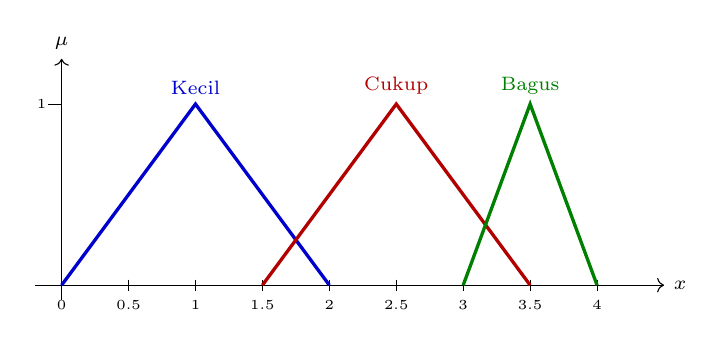
\begin{tikzpicture}[x=1.7cm, y=2.3cm, font=\scriptsize]
  \draw[->] (-0.2,0) -- (4.5,0) node[right] {$x$};
  \draw[->] (0,-0.08) -- (0,1.25) node[above] {$\mu$};
  \foreach \v in {0,0.5,1,1.5,2,2.5,3,3.5,4}
    \draw (\v,0.03) -- (\v,-0.03) node[below,font=\tiny] {\v};
  \draw (-0.1,1) -- (0,1) node[left=2pt,font=\tiny] {$1$};
  % MF curves
  \draw[very thick,blue!80!black]   (0,0) -- (1,1) -- (2,0);
  \draw[very thick,red!70!black]    (1.5,0) -- (2.5,1) -- (3.5,0);
  \draw[very thick,green!50!black]  (3,0) -- (3.5,1) -- (4,0);
  % Labels
  \node[above,blue!80!black] at (1,1) {Kecil};
  \node[above,red!70!black]  at (2.5,1) {Cukup};
  \node[above,green!50!black] at (3.5,1) {Bagus};
\end{tikzpicture}
\caption{MF segitiga untuk variabel IP.}
\label{fig:mf-ip}
\end{figure}

% --- Gambar 2: MF Variabel Minat -------------------------------------
\begin{figure}[htbp]
\centering
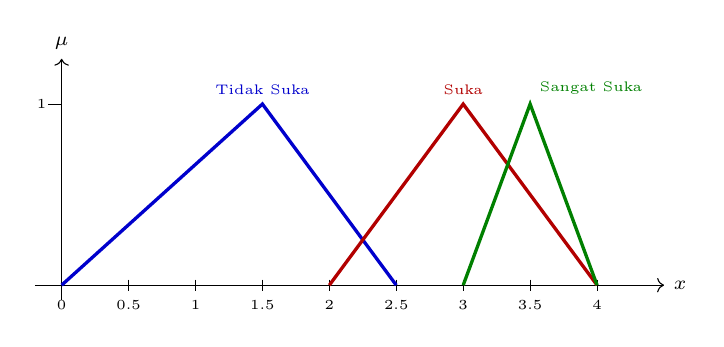
\begin{tikzpicture}[x=1.7cm, y=2.3cm, font=\scriptsize]
  \draw[->] (-0.2,0) -- (4.5,0) node[right] {$x$};
  \draw[->] (0,-0.08) -- (0,1.25) node[above] {$\mu$};
  \foreach \v in {0,0.5,1,1.5,2,2.5,3,3.5,4}
    \draw (\v,0.03) -- (\v,-0.03) node[below,font=\tiny] {\v};
  \draw (-0.1,1) -- (0,1) node[left=2pt,font=\tiny] {$1$};
  % MF curves
  \draw[very thick,blue!80!black]   (0,0) -- (1.5,1) -- (2.5,0);
  \draw[very thick,red!70!black]    (2,0) -- (3,1) -- (4,0);
  \draw[very thick,green!50!black]  (3,0) -- (3.5,1) -- (4,0);
  % Labels
  \node[above,blue!80!black] at (1.5,1) {\tiny Tidak Suka};
  \node[above,red!70!black]  at (3,1) {\tiny Suka};
  \node[above right,green!50!black,font=\tiny] at (3.5,1) {Sangat Suka};
\end{tikzpicture}
\caption{MF segitiga untuk variabel Minat.}
\label{fig:mf-minat}
\end{figure}

\subsection{Variabel Output: Nilai Kelayakan (NK)}

Semesta pembicaraan: $[0,\;100]$.

\begin{table}[htbp]
\centering\caption{MF variabel output NK.}
\label{tab:mf-nk}
\begin{tabular}{@{}lc@{}}
\toprule
Himpunan & $(a,\,b,\,c)$ \\
\midrule
Rendah & $(0,\;25,\;50)$ \\
Sedang & $(25,\;50,\;75)$ \\
Tinggi & $(50,\;75,\;100)$ \\
\bottomrule
\end{tabular}
\end{table}

% --- Gambar 3: MF Output NK ------------------------------------------
\begin{figure}[htbp]
\centering
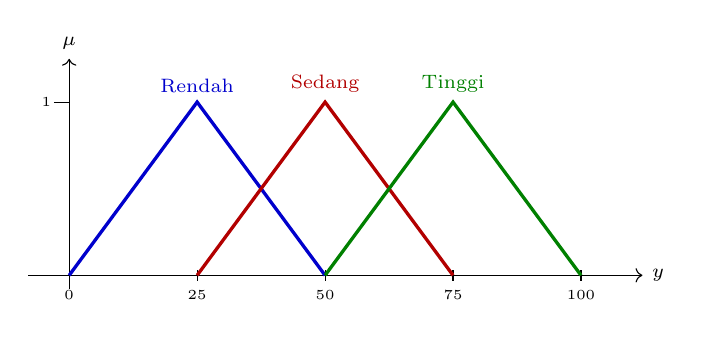
\begin{tikzpicture}[x=0.065cm, y=2.2cm, font=\scriptsize]
  \draw[->] (-8,0) -- (112,0) node[right] {$y$};
  \draw[->] (0,-0.08) -- (0,1.25) node[above] {$\mu$};
  \foreach \v in {0,25,50,75,100}
    \draw (\v,0.03) -- (\v,-0.03) node[below,font=\tiny] {\v};
  \draw (-3,1) -- (0,1) node[left=3pt,font=\tiny] {$1$};
  \draw[very thick,blue!80!black]   (0,0) -- (25,1) -- (50,0);
  \draw[very thick,red!70!black]    (25,0) -- (50,1) -- (75,0);
  \draw[very thick,green!50!black]  (50,0) -- (75,1) -- (100,0);
  \node[above,blue!80!black] at (25,1) {Rendah};
  \node[above,red!70!black]  at (50,1) {Sedang};
  \node[above,green!50!black] at (75,1) {Tinggi};
\end{tikzpicture}
\caption{MF segitiga untuk variabel output Nilai Kelayakan (NK).}
\label{fig:mf-nk}
\end{figure}

% =====================================================================
\section{Fuzzy Rules}
\label{sec:rules}
% =====================================================================

Sistem dirancang dengan 9 aturan fuzzy yang mencakup semua kombinasi
$3 \times 3$ dari himpunan IP dan Minat (Tabel~\ref{tab:rules}).

\begin{table}[htbp]
\centering\caption{Matriks 9 fuzzy rules (baris: IP, kolom: Minat).}
\label{tab:rules}
\begin{tabular}{@{}lccc@{}}
\toprule
\textbf{IP\textbackslash Minat} & \textbf{Tidak Suka} & \textbf{Suka} & \textbf{Sangat Suka} \\
\midrule
Kecil  & Rendah\,(R1) & Rendah\,(R2) & Sedang\,(R3) \\
Cukup  & Rendah\,(R4) & Sedang\,(R5) & Tinggi\,(R6) \\
Bagus  & Sedang\,(R7) & Tinggi\,(R8) & Tinggi\,(R9) \\
\bottomrule
\end{tabular}
\end{table}

\subsection{Justifikasi Setiap Rule}

\begin{enumerate}[nosep]
  \item \textbf{R1} (Kecil $\times$ Tidak Suka $\to$ Rendah):
        IP rendah dan tidak berminat --- tidak ada alasan untuk
        merekomendasikan.
  \item \textbf{R2} (Kecil $\times$ Suka $\to$ Rendah):
        Meskipun ada minat, IP rendah menunjukkan syarat akademik
        belum terpenuhi; risiko kegagalan tinggi.
  \item \textbf{R3} (Kecil $\times$ Sangat Suka $\to$ Sedang):
        Minat sangat kuat memberi peluang; output Sedang (bukan
        Rendah) memberi kesempatan bagi mahasiswa yang berpotensi
        meningkatkan IP.
  \item \textbf{R4} (Cukup $\times$ Tidak Suka $\to$ Rendah):
        IP memadai tetapi minat terlalu rendah --- konsentrasi
        tanpa minat cenderung berujung ketidakselesaan.
  \item \textbf{R5} (Cukup $\times$ Suka $\to$ Sedang):
        Keseimbangan moderat: IP dan minat keduanya cukup tetapi
        belum menonjol.
  \item \textbf{R6} (Cukup $\times$ Sangat Suka $\to$ Tinggi):
        Minat yang sangat kuat mengkompensasi IP yang hanya cukup;
        motivasi tinggi sering menghasilkan performa baik.
  \item \textbf{R7} (Bagus $\times$ Tidak Suka $\to$ Sedang):
        \textbf{Aturan kunci}: IP tinggi tanpa minat tidak cukup
        untuk rekomendasi Tinggi. Pengalaman menunjukkan bahwa
        ketidaksesuaian minat menyebabkan ketidakpuasan dan risiko
        drop-out meskipun nilai bagus. Hanya Sedang.
  \item \textbf{R8} (Bagus $\times$ Suka $\to$ Tinggi):
        Kombinasi ideal --- kapabilitas akademik didukung minat
        yang kuat.
  \item \textbf{R9} (Bagus $\times$ Sangat Suka $\to$ Tinggi):
        Rekomendasi terkuat; baik akademik maupun minat optimal.
\end{enumerate}

\noindent
\textbf{Prinsip desain:}
\begin{itemize}[nosep,leftmargin=*]
  \item IP rendah ($\leq 2$) $\Rightarrow$ output tidak lebih dari Sedang,
        karena syarat akademik fundamental belum terpenuhi.
  \item Minat rendah (Tidak Suka) $\Rightarrow$ batasi output, karena
        ketidaksesuaian minat berisiko tinggi.
  \item Aturan R7 adalah \emph{differentiator kunci} yang memastikan
        IP tinggi saja tidak cukup tanpa disertai minat.
\end{itemize}

% =====================================================================
\section{Inferensi Mamdani dan Defuzzifikasi COG}
\label{sec:inferensi}
% =====================================================================

\subsection{Pemilihan Metode Inferensi}

Dari tiga metode inferensi fuzzy yang umum (Mamdani, Sugeno, Tsukamoto),
penulis memilih \textbf{metode Mamdani} dengan justifikasi sebagai berikut:

\begin{enumerate}[nosep]
  \item \textbf{Intuitif dan mudah divisualisasikan:}
        Mamdani menghasilkan area fuzzy output yang dapat divisualisasikan
        secara eksplisit (Gambar~\ref{fig:agregasi-target}), sehingga
        proses pengambilan keputusan mudah dipahami dan dijelaskan.
  \item \textbf{Cocok untuk SPK:} Sistem Pendukung Keputusan memerlukan
        transparansi; Mamdani memungkinkan tracing setiap langkah
        dari fuzzifikasi hingga defuzzifikasi.
  \item \textbf{Konsistensi:} Metode ini konsisten dengan materi
        perkuliahan dan tugas mandiri pertemuan 7 \cite{mulki2026}.
\end{enumerate}

\noindent
Tahapan Mamdani yang diterapkan:
\begin{enumerate}[nosep]
  \item \textbf{Fuzzifikasi:} Pemetaan nilai crisp ke derajat keanggotaan.
  \item \textbf{Evaluasi aturan:} $\alpha_i = \min(\mu_{\text{IP},i},\;
        \mu_{\text{Minat},i})$.
  \item \textbf{Implikasi:} $\mu'_i(y) = \min(\alpha_i,\;
        \mu_{\text{konsekuen}}(y))$ (clipping).
  \item \textbf{Agregasi:} $\mu_{\text{agg}}(y) = \max_i \mu'_i(y)$.
  \item \textbf{Defuzzifikasi COG:}
        $y^* = \dfrac{\int y\,\mu_{\text{agg}}(y)\,\mathrm{d}y}
                     {\int \mu_{\text{agg}}(y)\,\mathrm{d}y}$
\end{enumerate}

\subsection{Detail Perhitungan: Data Target \#20}

Sistem menjalankan FIS Mamdani secara terpisah untuk setiap KBK,
menghitung NK masing-masing, lalu merekomendasikan KBK dengan NK
tertinggi.

\subsubsection{KBK ITP: $IP=3.40$, $Minat=2.60$}

\textbf{Fuzzifikasi:}
\begin{align}
  \mu_{\text{Kecil}}(3.40) &= 0,\quad
  \mu_{\text{Cukup}}(3.40) = \tfrac{3.5-3.4}{3.5-2.5} = \mathbf{0.1}, \notag\\
  \mu_{\text{Bagus}}(3.40) &= \tfrac{3.4-3}{3.5-3} = \mathbf{0.8}. \notag
\end{align}
\begin{align}
  \mu_{\text{TS}}(2.60) &= 0,\quad
  \mu_{\text{Suka}}(2.60) = \tfrac{2.6-2}{3-2} = \mathbf{0.6}, \notag\\
  \mu_{\text{SS}}(2.60) &= 0. \notag
\end{align}

\textbf{Rules aktif:}
\begin{itemize}[nosep]
  \item R5 (Cukup $\times$ Suka $\to$ Sedang):
        $\alpha = \min(0.1;\;0.6) = 0.1$
  \item R8 (Bagus $\times$ Suka $\to$ Tinggi):
        $\alpha = \min(0.8;\;0.6) = 0.6$
\end{itemize}

Agregasi: $\max(\text{Sedang}@0.1,\;\text{Tinggi}@0.6)$.
Karena Tinggi mendominasi, COG $\approx 71.14$.

\subsubsection{KBK RPLD: $IP=3.52$, $Minat=2.80$}

\textbf{Fuzzifikasi:}
\begin{align}
  \mu_{\text{Cukup}}(3.52) &= 0,\quad
  \mu_{\text{Bagus}}(3.52) = \tfrac{4-3.52}{4-3.5} = \mathbf{0.96}. \notag\\
  \mu_{\text{Suka}}(2.80) &= \tfrac{2.8-2}{3-2} = \mathbf{0.8}. \notag
\end{align}

\textbf{Rule aktif:}
\begin{itemize}[nosep]
  \item R8 (Bagus $\times$ Suka $\to$ Tinggi):
        $\alpha = \min(0.96;\;0.8) = \mathbf{0.8}$
\end{itemize}

Hanya satu rule aktif: Tinggi dipotong pada $\alpha=0.8$.
Trapesium hasil implikasi: $(50,0)\!\to\!(70,0.8)\!\to\!(80,0.8)\!\to\!(100,0)$.
COG dari trapesium simetris = titik puncak $= \mathbf{75.00}$.

\subsubsection{KBK SKJK: $IP=3.65$, $Minat=1.50$}

\textbf{Fuzzifikasi:}
\begin{align}
  \mu_{\text{Bagus}}(3.65) &= \tfrac{4-3.65}{4-3.5} = \mathbf{0.7}. \notag\\
  \mu_{\text{TS}}(1.50) &= \tfrac{1.5-0}{1.5-0} = \mathbf{1.0}
  \quad\text{(puncak)}. \notag
\end{align}

\textbf{Rule aktif:}
\begin{itemize}[nosep]
  \item R7 (Bagus $\times$ Tidak Suka $\to$ Sedang):
        $\alpha = \min(0.7;\;1.0) = \mathbf{0.7}$
\end{itemize}

Hanya satu rule aktif: Sedang dipotong pada $\alpha=0.7$.
COG dari trapesium simetris = titik puncak $= \mathbf{50.00}$.

% --- Gambar 4: Fuzzifikasi detail data target #20 --------------------
\begin{figure*}[htbp]
\centering
% (a) IP fuzzifikasi
\begin{minipage}[t]{0.47\textwidth}
\centering\textbf{(a) Fuzzifikasi IP --- 3 KBK}\par\smallskip
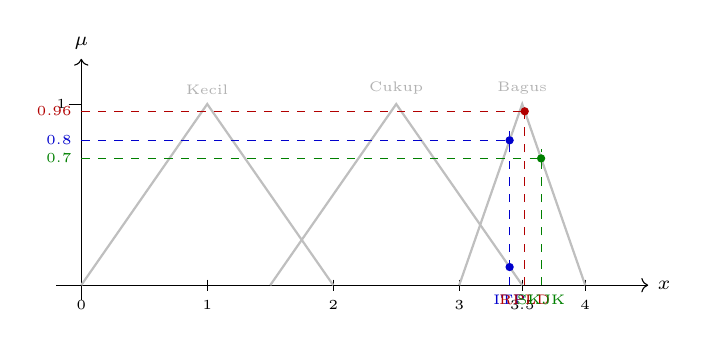
\begin{tikzpicture}[x=1.6cm, y=2.3cm, font=\scriptsize]
  \draw[->] (-0.2,0) -- (4.5,0) node[right] {$x$};
  \draw[->] (0,-0.08) -- (0,1.25) node[above] {$\mu$};
  \foreach \v in {0,1,2,3,3.5,4}
    \draw (\v,0.03) -- (\v,-0.03) node[below,font=\tiny] {\v};
  \draw (-0.1,1) -- (0,1) node[left=2pt,font=\tiny] {$1$};
  % MF curves (light)
  \draw[thick,gray!50] (0,0) -- (1,1) -- (2,0);
  \draw[thick,gray!50] (1.5,0) -- (2.5,1) -- (3.5,0);
  \draw[thick,gray!50] (3,0) -- (3.5,1) -- (4,0);
  % ITP: IP=3.40 → μ_Cukup=0.1, μ_Bagus=0.8
  \draw[dashed,blue!80!black] (3.4,0) -- (3.4,0.85);
  \fill[blue!80!black] (3.4,0.8) circle (1.5pt);
  \fill[blue!80!black] (3.4,0.1) circle (1.5pt);
  \draw[dashed,blue!80!black] (0,0.8) -- (3.4,0.8);
  \node[left,blue!80!black,font=\tiny] at (0,0.8) {$0.8$};
  \node[below,blue!80!black,font=\tiny] at (3.4,0) {ITP};
  % RPLD: IP=3.52 → μ_Bagus=0.96
  \draw[dashed,red!70!black] (3.52,0) -- (3.52,0.99);
  \fill[red!70!black] (3.52,0.96) circle (1.5pt);
  \draw[dashed,red!70!black] (0,0.96) -- (3.52,0.96);
  \node[left,red!70!black,font=\tiny] at (0,0.96) {$0.96$};
  \node[below,red!70!black,font=\tiny] at (3.52,0) {RPLD};
  % SKJK: IP=3.65 → μ_Bagus=0.7
  \draw[dashed,green!50!black] (3.65,0) -- (3.65,0.75);
  \fill[green!50!black] (3.65,0.7) circle (1.5pt);
  \draw[dashed,green!50!black] (0,0.7) -- (3.65,0.7);
  \node[left,green!50!black,font=\tiny] at (0,0.7) {$0.7$};
  \node[below,green!50!black,font=\tiny] at (3.65,0) {SKJK};
  % MF labels
  \node[above,gray!60] at (1,1) {\tiny Kecil};
  \node[above,gray!60] at (2.5,1) {\tiny Cukup};
  \node[above,gray!60] at (3.5,1) {\tiny Bagus};
\end{tikzpicture}
\end{minipage}\hfill
% (b) Minat fuzzifikasi
\begin{minipage}[t]{0.47\textwidth}
\centering\textbf{(b) Fuzzifikasi Minat --- 3 KBK}\par\smallskip
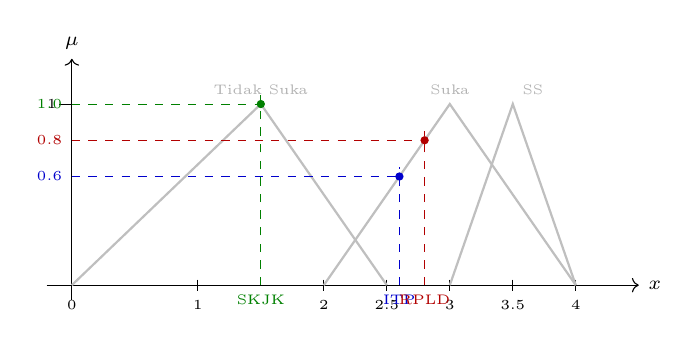
\begin{tikzpicture}[x=1.6cm, y=2.3cm, font=\scriptsize]
  \draw[->] (-0.2,0) -- (4.5,0) node[right] {$x$};
  \draw[->] (0,-0.08) -- (0,1.25) node[above] {$\mu$};
  \foreach \v in {0,1,2,2.5,3,3.5,4}
    \draw (\v,0.03) -- (\v,-0.03) node[below,font=\tiny] {\v};
  \draw (-0.1,1) -- (0,1) node[left=2pt,font=\tiny] {$1$};
  % MF curves (light)
  \draw[thick,gray!50] (0,0) -- (1.5,1) -- (2.5,0);
  \draw[thick,gray!50] (2,0) -- (3,1) -- (4,0);
  \draw[thick,gray!50] (3,0) -- (3.5,1) -- (4,0);
  % ITP: Minat=2.60 → μ_Suka=0.6
  \draw[dashed,blue!80!black] (2.6,0) -- (2.6,0.65);
  \fill[blue!80!black] (2.6,0.6) circle (1.5pt);
  \draw[dashed,blue!80!black] (0,0.6) -- (2.6,0.6);
  \node[left,blue!80!black,font=\tiny] at (0,0.6) {$0.6$};
  \node[below,blue!80!black,font=\tiny] at (2.6,0) {ITP};
  % RPLD: Minat=2.80 → μ_Suka=0.8
  \draw[dashed,red!70!black] (2.8,0) -- (2.8,0.85);
  \fill[red!70!black] (2.8,0.8) circle (1.5pt);
  \draw[dashed,red!70!black] (0,0.8) -- (2.8,0.8);
  \node[left,red!70!black,font=\tiny] at (0,0.8) {$0.8$};
  \node[below,red!70!black,font=\tiny] at (2.8,0) {RPLD};
  % SKJK: Minat=1.50 → μ_TS=1.0 (puncak)
  \draw[dashed,green!50!black] (1.5,0) -- (1.5,1.05);
  \fill[green!50!black] (1.5,1.0) circle (1.5pt);
  \draw[dashed,green!50!black] (0,1.0) -- (1.5,1.0);
  \node[left,green!50!black,font=\tiny] at (0,1.0) {$1.0$};
  \node[below,green!50!black,font=\tiny] at (1.5,0) {SKJK};
  % MF labels
  \node[above,gray!60] at (1.5,1) {\tiny Tidak Suka};
  \node[above,gray!60] at (3,1) {\tiny Suka};
  \node[above right,gray!60,font=\tiny] at (3.5,1) {SS};
\end{tikzpicture}
\end{minipage}
\caption{Fuzzifikasi data target \#20: titik-titik menunjukkan nilai crisp
setiap KBK pada kurva MF. \textbf{(a)} IP: ketiganya masuk himpunan Bagus
dengan $\mu$ berbeda. \textbf{(b)} Minat: ITP dan RPLD masuk Suka, sedangkan
SKJK tepat di puncak Tidak Suka ($\mu=1.0$).}
\label{fig:fuzzifikasi-target}
\end{figure*}

% --- Gambar 5: Diagram alir Mamdani ----------------------------------
\begin{figure*}[htbp]
\centering
\resizebox{\textwidth}{!}{%
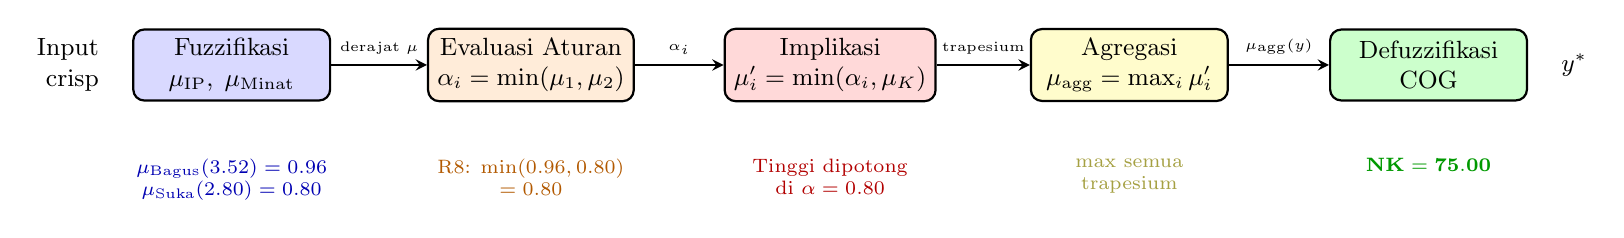
\begin{tikzpicture}[
  box/.style={draw, rounded corners, minimum width=2.5cm, minimum height=0.9cm,
              font=\small, align=center, thick},
  arr/.style={->, thick, >=stealth},
  lbl/.style={font=\tiny, midway, above}
]
  \node[box, fill=blue!15]   (fuzz)  at (0,0)    {Fuzzifikasi\\$\mu_{\text{IP}},\;\mu_{\text{Minat}}$};
  \node[box, fill=orange!15] (eval)  at (3.8,0)  {Evaluasi Aturan\\$\alpha_i = \min(\mu_1,\mu_2)$};
  \node[box, fill=red!15]    (impl)  at (7.6,0)  {Implikasi\\$\mu'_i = \min(\alpha_i,\mu_K)$};
  \node[box, fill=yellow!20] (agg)   at (11.4,0) {Agregasi\\$\mu_{\text{agg}} = \max_i \mu'_i$};
  \node[box, fill=green!20]  (cog)   at (15.2,0) {Defuzzifikasi\\COG};
  \draw[arr] (fuzz) -- (eval) node[lbl] {derajat $\mu$};
  \draw[arr] (eval) -- (impl) node[lbl] {$\alpha_i$};
  \draw[arr] (impl) -- (agg)  node[lbl] {trapesium};
  \draw[arr] (agg)  -- (cog)  node[lbl] {$\mu_{\text{agg}}(y)$};
  % Input/output labels
  \node[font=\small, left=0.3cm of fuzz, align=right] {Input\\crisp};
  \node[font=\small, right=0.3cm of cog] {$y^*$};
  % Example below
  \node[font=\scriptsize, text=blue!70!black, below=0.6cm of fuzz, align=center]
    {$\mu_{\text{Bagus}}(3.52)=0.96$\\$\mu_{\text{Suka}}(2.80)=0.80$};
  \node[font=\scriptsize, text=orange!70!black, below=0.6cm of eval, align=center]
    {R8: $\min(0.96,0.80)$\\$= 0.80$};
  \node[font=\scriptsize, text=red!70!black, below=0.6cm of impl, align=center]
    {Tinggi dipotong\\di $\alpha=0.80$};
  \node[font=\scriptsize, text=yellow!60!black, below=0.6cm of agg, align=center]
    {$\max$ semua\\trapesium};
  \node[font=\scriptsize, text=green!60!black, below=0.6cm of cog, align=center]
    {$\mathbf{NK=75.00}$};
\end{tikzpicture}%
}
\caption{Diagram alir proses Mamdani dengan contoh data RPLD \#20.}
\label{fig:flowchart}
\end{figure*}

% --- Gambar 6: Agregasi data target #20 untuk 3 KBK -----------------
\begin{figure*}[htbp]
\centering
% ITP
\begin{minipage}[t]{0.32\textwidth}
\centering\textbf{(a) KBK ITP}\par
$\text{NK}_{\text{ITP}} = 71.14$\par\smallskip
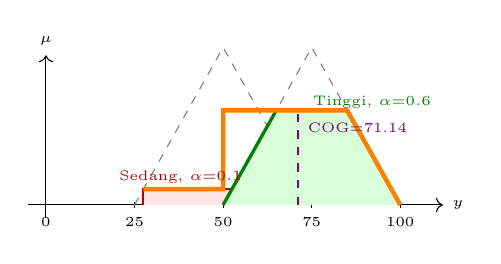
\begin{tikzpicture}[x=0.045cm, y=2cm, font=\tiny]
  \draw[->] (-5,0) -- (112,0) node[right] {$y$};
  \draw[->] (0,-0.08) -- (0,0.95) node[above] {$\mu$};
  \foreach \v in {0,25,50,75,100}
    \draw (\v,0.02) -- (\v,-0.02) node[below] {\v};
  % Sedang@0.1
  \draw[dashed,gray] (25,0) -- (50,1) -- (75,0);
  % Tinggi@0.6
  \draw[dashed,gray] (50,0) -- (75,1) -- (100,0);
  % Sedang clipped at 0.1
  \fill[red!10] (27.5,0) -- (27.5,0.1) -- (72.5,0.1) -- (72.5,0) -- cycle;
  \draw[thick,red!70!black] (27.5,0) -- (27.5,0.1) -- (72.5,0.1) -- (72.5,0);
  % Tinggi clipped at 0.6
  \fill[green!15] (50,0) -- (65,0.6) -- (85,0.6) -- (100,0) -- cycle;
  \draw[very thick,green!50!black] (50,0) -- (65,0.6) -- (85,0.6) -- (100,0);
  % Aggregate
  \draw[ultra thick,orange] (27.5,0.1) -- (50,0.1) -- (50,0.6) -- (65,0.6)
    -- (85,0.6) -- (100,0);
  % COG
  \draw[dashed,violet] (71.14,0) -- (71.14,0.6);
  \node[violet,above right] at (71.14,0.4) {\tiny COG=71.14};
  % Labels
  \node[red!70!black] at (38,0.18) {\tiny Sedang, $\alpha{=}0.1$};
  \node[green!50!black] at (92,0.65) {\tiny Tinggi, $\alpha{=}0.6$};
\end{tikzpicture}
\end{minipage}\hfill
% RPLD
\begin{minipage}[t]{0.32\textwidth}
\centering\textbf{(b) KBK RPLD}\par
$\text{NK}_{\text{RPLD}} = 75.00$\par\smallskip
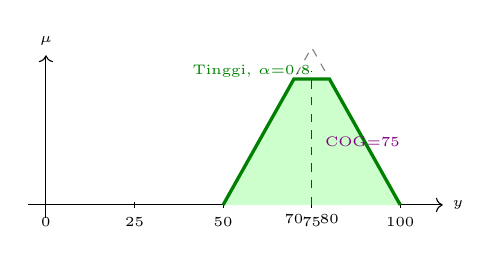
\begin{tikzpicture}[x=0.045cm, y=2cm, font=\tiny]
  \draw[->] (-5,0) -- (112,0) node[right] {$y$};
  \draw[->] (0,-0.08) -- (0,0.95) node[above] {$\mu$};
  \foreach \v in {0,25,50,75,100}
    \draw (\v,0.02) -- (\v,-0.02) node[below] {\v};
  % Tinggi original
  \draw[dashed,gray] (50,0) -- (75,1) -- (100,0);
  % Tinggi clipped at 0.8
  \fill[green!20] (50,0) -- (70,0.8) -- (80,0.8) -- (100,0) -- cycle;
  \draw[very thick,green!50!black] (50,0) -- (70,0.8) -- (80,0.8) -- (100,0);
  % COG
  \draw[dashed,violet] (75,0) -- (75,0.85);
  \node[violet,right] at (76,0.4) {\tiny COG=75};
  \node[green!50!black] at (58,0.85) {\tiny Tinggi, $\alpha{=}0.8$};
  \node[below] at (70,0) {$70$};
  \node[below] at (80,0) {$80$};
\end{tikzpicture}
\end{minipage}\hfill
% SKJK
\begin{minipage}[t]{0.32\textwidth}
\centering\textbf{(c) KBK SKJK}\par
$\text{NK}_{\text{SKJK}} = 50.00$\par\smallskip
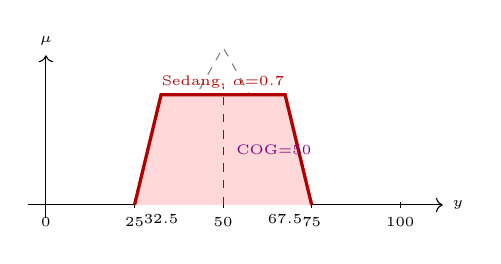
\begin{tikzpicture}[x=0.045cm, y=2cm, font=\tiny]
  \draw[->] (-5,0) -- (112,0) node[right] {$y$};
  \draw[->] (0,-0.08) -- (0,0.95) node[above] {$\mu$};
  \foreach \v in {0,25,50,75,100}
    \draw (\v,0.02) -- (\v,-0.02) node[below] {\v};
  % Sedang original
  \draw[dashed,gray] (25,0) -- (50,1) -- (75,0);
  % Sedang clipped at 0.7
  \fill[red!15] (25,0) -- (32.5,0.7) -- (67.5,0.7) -- (75,0) -- cycle;
  \draw[very thick,red!70!black] (25,0) -- (32.5,0.7) -- (67.5,0.7) -- (75,0);
  % COG
  \draw[dashed,violet] (50,0) -- (50,0.75);
  \node[violet,right] at (51,0.35) {\tiny COG=50};
  \node[red!70!black] at (50,0.78) {\tiny Sedang, $\alpha{=}0.7$};
  \node[below] at (32.5,0) {$32.5$};
  \node[below] at (67.5,0) {$67.5$};
\end{tikzpicture}
\end{minipage}
\caption{Agregasi Mamdani dan COG untuk data target \#20 pada ketiga KBK.
NK$_{\text{RPLD}}=75 > $ NK$_{\text{ITP}}=71.14 > $ NK$_{\text{SKJK}}=50$
$\Rightarrow$ rekomendasi: \textbf{RPLD}.}
\label{fig:agregasi-target}
\end{figure*}

\subsubsection{Perbandingan NK Data \#20}

\begin{table}[htbp]
\centering\caption{Perbandingan NK untuk data target \#20.}
\label{tab:target}
\begin{tabular}{@{}lccccc@{}}
\toprule
KBK & IP & Minat & Rule Aktif & $\alpha$ & NK (COG) \\
\midrule
ITP  & $3.40$ & $2.60$ & R5, R8 & $0.1;\;0.6$ & $71.14$ \\
\textbf{RPLD} & $\mathbf{3.52}$ & $\mathbf{2.80}$
  & \textbf{R8} & $\mathbf{0.8}$ & $\mathbf{75.00}$ \\
SKJK & $3.65$ & $1.50$ & R7     & $0.7$ & $50.00$ \\
\bottomrule
\end{tabular}
\end{table}

\begin{gather*}
  \text{NK}_{\text{RPLD}} = 75.00 > \text{NK}_{\text{ITP}} = 71.14 > \text{NK}_{\text{SKJK}} = 50.00 \\[4pt]
  \boxed{\textbf{Rekomendasi: RPLD} \;\checkmark}
\end{gather*}

% --- Gambar 7: Bar chart NK comparison ------------------------------
\begin{figure}[htbp]
\centering
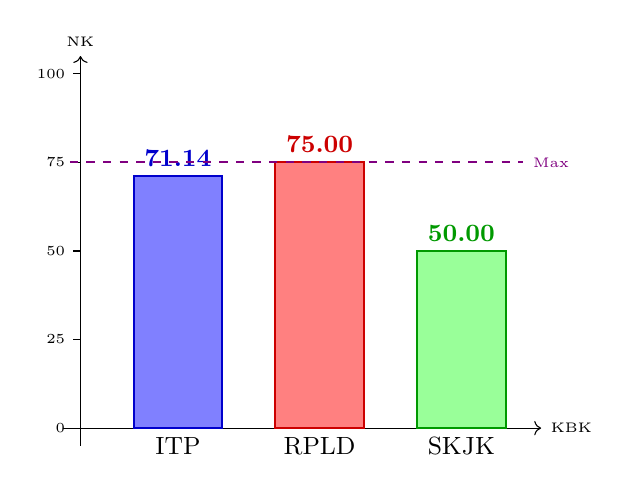
\begin{tikzpicture}[x=0.045cm, y=0.045cm, font=\scriptsize]
  % Axes
  \draw[->] (-5,0) -- (130,0) node[right] {\tiny KBK};
  \draw[->] (0,-5) -- (0,105) node[above] {\tiny NK};
  \foreach \v in {0,25,50,75,100}
    \draw (-2,\v) -- (0,\v) node[left=2pt,font=\tiny] {\v};
  % ITP bar
  \fill[blue!50] (15,0) rectangle (40,71.14);
  \draw[thick,blue!80!black] (15,0) rectangle (40,71.14);
  \node[above,blue!80!black,font=\small\bfseries] at (27.5,71.14) {71.14};
  \node[below,font=\small] at (27.5,0) {ITP};
  % RPLD bar
  \fill[red!50] (55,0) rectangle (80,75);
  \draw[thick,red!80!black] (55,0) rectangle (80,75);
  \node[above,red!80!black,font=\small\bfseries] at (67.5,75) {75.00};
  \node[below,font=\small] at (67.5,0) {RPLD};
  % SKJK bar
  \fill[green!40] (95,0) rectangle (120,50);
  \draw[thick,green!60!black] (95,0) rectangle (120,50);
  \node[above,green!60!black,font=\small\bfseries] at (107.5,50) {50.00};
  \node[below,font=\small] at (107.5,0) {SKJK};
  % NK threshold line
  \draw[dashed,thick,violet] (-3,75) -- (125,75);
  \node[right,violet,font=\tiny] at (125,75) {Max};
\end{tikzpicture}
\caption{Perbandingan Nilai Kelayakan (NK) untuk data target \#20.
RPLD memiliki NK tertinggi ($75.00$) dan direkomendasikan.}
\label{fig:bar-nk}
\end{figure}

\vspace{0.5em}
\noindent\textbf{Analisis mengapa RPLD menang:}
\begin{itemize}[nosep,leftmargin=*]
  \item \textbf{SKJK} memiliki IP tertinggi ($3.65$) tetapi minat
        sangat rendah ($1.50$). Aturan R7 membatasi output menjadi
        \emph{Sedang} (NK = 50) karena minat yang tidak memadai.
  \item \textbf{ITP} memiliki kombinasi cukup baik ($3.40$; $2.60$)
        tetapi $\mu_{\text{Suka}}(2.60) = 0.6$ lebih rendah dari
        $\mu_{\text{Suka}}(2.80) = 0.8$ milik RPLD, sehingga
        $\alpha_{\text{R8}}$ untuk ITP hanya 0.6.
  \item \textbf{RPLD} memiliki kombinasi terbaik: IP tinggi ($3.52$,
        $\mu_{\text{Bagus}}=0.96$) dan minat cukup kuat ($2.80$,
        $\mu_{\text{Suka}}=0.8$), menghasilkan $\alpha=0.8$ pada
        rule R8 yang mengarah ke output Tinggi.
\end{itemize}

% =====================================================================
\section{Hasil dan Verifikasi}
\label{sec:hasil}
% =====================================================================

Simulasi Python (\texttt{sim\_fuzzy\_spk.py}) mengimplementasikan FIS
Mamdani secara numerik dengan $n=10\,001$ titik diskritisasi.
Tabel~\ref{tab:hasil} menyajikan hasil lengkap untuk 20 data.

\subsection{Analisis Decision Boundary}
\label{subsec:decision-boundary}

Decision boundary (Gambar~\ref{fig:decision-boundary}) memetakan
Nilai Kelayakan sebagai fungsi dari dua variabel input secara
serentak. Sumbu horizontal merepresentasikan IPK ($0$--$4$), sumbu
vertikal merepresentasikan Minat ($0$--$4$), dan warna menunjukkan
NK: \textcolor{red}{merah} untuk NK rendah, \textcolor{green}{hijau}
untuk NK tinggi. Garis putus-putus menandai \emph{threshold}
NK$=50$ (batas Rendah/Sedang) dan NK$=75$ (batas Sedang/Tinggi).

\noindent\textbf{Cara membaca chart untuk data target \#20:}
\begin{itemize}[nosep,leftmargin=*]
  \item \textbf{SKJK} ($\circ$): berada di kanan bawah (IP$=3.65$,
        Minat$=1.50$) --- zona merah/kuning. IP tinggi namun minat
        sangat rendah menyebabkan NK hanya $50$ (Sedang), karena
        rule R7 membatasi output.
  \item \textbf{ITP} ($\square$): berada di tengah (IP$=3.40$,
        Minat$=2.60$) --- zona kuning/hijau muda. Kombinasi cukup
        baik, NK $=71.14$.
  \item \textbf{RPLD} ($\triangle$): berada di kanan atas (IP$=3.52$,
        Minat$=2.80$) --- zona hijau tua. Kombinasi terbaik,
        NK $=75.00$ (tertinggi).
\end{itemize}

\noindent\textbf{Interpretasi visual:} Chart ini menunjukkan bahwa
NK tinggi (hijau) \emph{hanya} tercapai ketika kedua variabel
memadai. Area kanan bawah (IP tinggi, Minat rendah) tetap berwarna
kuning/merah --- inilah konsekuensi dari rule R7. Tanpa rule ini,
seluruh sisi kanan chart akan berwarna hijau tanpa memandang minat.

% --- Gambar Decision Boundary ----------------------------------------
\begin{figure}[htbp]
\centering
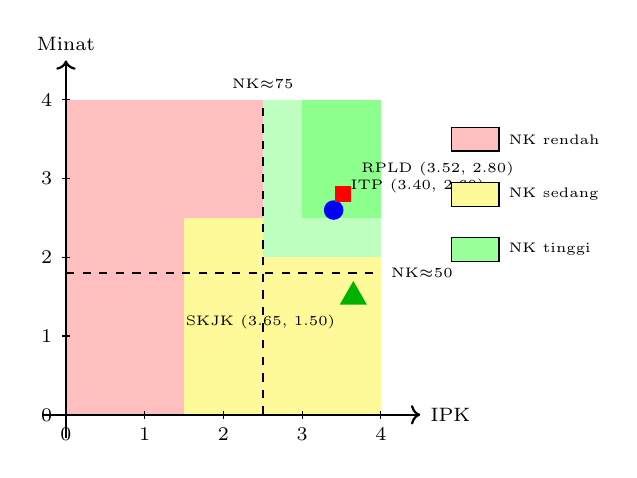
\begin{tikzpicture}[font=\scriptsize]
  % Simulated contour zones
  \fill[red!25]     (0,0) rectangle (4,4);
  \fill[yellow!40]  (1.5,0) -- (4,0) -- (4,2.5) -- (1.5,2.5) -- cycle;
  \fill[green!25]   (2.5,2) -- (4,2) -- (4,4) -- (2.5,4) -- cycle;
  \fill[green!45]   (3,2.5) -- (4,2.5) -- (4,4) -- (3,4) -- cycle;

  % Axes
  \draw[->,thick] (-0.3,0) -- (4.5,0) node[right] {IPK};
  \draw[->,thick] (0,-0.3) -- (0,4.5) node[above] {Minat};
  \foreach \v in {0,1,2,3,4} {
    \draw (\v,0.05) -- (\v,-0.05) node[below] {\v};
    \draw (0.05,\v) -- (-0.05,\v) node[left] {\v};
  }

  % Threshold lines
  \draw[dashed,thick] (0,1.8) -- (4,1.8)
    node[right,font=\tiny] {NK$\approx$50};
  \draw[dashed,thick] (2.5,0) -- (2.5,4)
    node[above,font=\tiny] {NK$\approx$75};

  % Data #20 markers
  \node[circle,fill=blue,inner sep=2.5pt,
    label={[font=\tiny]above right:{ITP (3.40, 2.60)}}] at (3.40,2.60) {};
  \node[regular polygon, regular polygon sides=4,fill=red,inner sep=2pt,
    label={[font=\tiny]above right:{RPLD (3.52, 2.80)}}] at (3.52,2.80) {};
  \node[regular polygon, regular polygon sides=3,fill=green!70!black,inner sep=2pt,
    label={[font=\tiny]below left:{SKJK (3.65, 1.50)}}] at (3.65,1.50) {};

  % Color legend
  \node[fill=red!25,draw,minimum width=0.6cm,minimum height=0.3cm] at (5.2,3.5) {};
  \node[right,font=\tiny] at (5.5,3.5) {NK rendah};
  \node[fill=yellow!40,draw,minimum width=0.6cm,minimum height=0.3cm] at (5.2,2.8) {};
  \node[right,font=\tiny] at (5.5,2.8) {NK sedang};
  \node[fill=green!40,draw,minimum width=0.6cm,minimum height=0.3cm] at (5.2,2.1) {};
  \node[right,font=\tiny] at (5.5,2.1) {NK tinggi};
\end{tikzpicture}
\caption{Decision boundary NK(IPK,\,Minat): zona hijau = kelayakan
tinggi hanya tercapai bila IPK dan Minat keduanya memadai.
Titik RPLD berada di zona hijau, sedangkan SKJK jatuh di zona
merah/kuning akibat rule R7.}
\label{fig:decision-boundary}
\end{figure}

\begin{table*}[htbp]
\centering\caption{Hasil rekomendasi FIS Mamdani untuk 20 data survei.}
\label{tab:hasil}
\small
\begin{tabular}{@{}c cc cc cc c c@{}}
\toprule
\multirow{2}{*}{No} & \multicolumn{2}{c}{ITP} & \multicolumn{2}{c}{RPLD}
  & \multicolumn{2}{c}{SKJK} & \multirow{2}{*}{Pilihan} & \multirow{2}{*}{Rekomendasi} \\
\cmidrule(lr){2-3}\cmidrule(lr){4-5}\cmidrule(lr){6-7}
  & NK & & NK & & NK & & & \\
\midrule
1  & 75.00 & & 39.23 & & 25.00 & & ITP  & \textbf{ITP}\,$\checkmark$ \\
2  & 75.00 & & 45.10 & & 25.00 & & ITP  & \textbf{ITP}\,$\checkmark$ \\
3  & 75.00 & & 54.17 & & 33.33 & & ITP  & \textbf{ITP}\,$\checkmark$ \\
4  & 75.00 & & 45.10 & & 25.00 & & ITP  & \textbf{ITP}\,$\checkmark$ \\
5  & 75.00 & & 46.91 & & 25.00 & & ITP  & \textbf{ITP}\,$\checkmark$ \\
6  & 75.00 & & 68.27 & & 25.00 & & ITP  & \textbf{ITP}\,$\checkmark$ \\
7  & 75.00 & & 33.33 & & 25.00 & & ITP  & \textbf{ITP}\,$\checkmark$ \\
\midrule
8  & 25.00 & & 75.00 & & 25.00 & & RPLD & \textbf{RPLD}\,$\checkmark$ \\
9  & 25.00 & & 75.00 & & 59.38 & & RPLD & \textbf{RPLD}\,$\checkmark$ \\
10 & 25.00 & & 75.00 & & 25.00 & & RPLD & \textbf{RPLD}\,$\checkmark$ \\
11 & 25.00 & & 75.00 & & 34.86 & & RPLD & \textbf{RPLD}\,$\checkmark$ \\
12 & 25.00 & & 75.00 & & 68.27 & & RPLD & \textbf{RPLD}\,$\checkmark$ \\
13 & 25.00 & & 75.00 & & 45.10 & & RPLD & \textbf{RPLD}\,$\checkmark$ \\
\midrule
14 & 25.00 & & 25.00 & & 75.00 & & SKJK & \textbf{SKJK}\,$\checkmark$ \\
15 & 25.00 & & 25.00 & & 75.00 & & SKJK & \textbf{SKJK}\,$\checkmark$ \\
16 & 25.00 & & 25.00 & & 75.00 & & SKJK & \textbf{SKJK}\,$\checkmark$ \\
17 & 25.00 & & 25.00 & & 75.00 & & SKJK & \textbf{SKJK}\,$\checkmark$ \\
18 & 25.00 & & 25.00 & & 75.00 & & SKJK & \textbf{SKJK}\,$\checkmark$ \\
19 & 25.00 & & 25.00 & & 75.00 & & SKJK & \textbf{SKJK}\,$\checkmark$ \\
\midrule
\textbf{20} & \textbf{71.14} & & \textbf{75.00} & & \textbf{50.00} &
  & \textbf{?} & \textbf{RPLD}\,$\checkmark$ \\
\bottomrule
\end{tabular}
\end{table*}

\begin{itemize}[nosep]
  \item Akurasi pada 19 data latih: \textbf{19/19 = 100\,\%}.
  \item Data target \#20 berhasil merekomendasikan \textbf{RPLD}
        sesuai persyaratan soal ujian.
\end{itemize}

% =====================================================================
\section{Kesimpulan}
\label{sec:kesimpulan}
% =====================================================================

\begin{enumerate}[nosep]
  \item Fuzzifikasi dirancang dengan 3 himpunan segitiga untuk setiap
        variabel (IP: Kecil, Cukup, Bagus; Minat: Tidak Suka, Suka,
        Sangat Suka; NK: Rendah, Sedang, Tinggi). Pemilihan kurva
        segitiga didasarkan pada kesederhanaan, efisiensi komputasi,
        dan jangkauan yang sesuai dengan distribusi data survei.
  \item Sembilan fuzzy rules dirancang berdasarkan prinsip bahwa
        \emph{baik IP maupun minat harus memadai untuk rekomendasi
        tinggi}. Aturan R7 (Bagus $\times$ Tidak Suka $\to$ Sedang)
        menjadi kunci diferensiasi yang memastikan IP tinggi tanpa
        minat tidak langsung menghasilkan rekomendasi Tinggi.
  \item Metode Mamdani dipilih karena intuitif, mudah divisualisasikan,
        dan cocok untuk SPK. Defuzzifikasi menggunakan COG.
  \item Verifikasi menunjukkan sistem berhasil merekomendasikan
        \textbf{RPLD} untuk data target \#20
        (NK$_{\text{RPLD}}=75.00 > $ NK$_{\text{ITP}}=71.14 > $
        NK$_{\text{SKJK}}=50.00$) dengan akurasi 100\,\% pada
        19 data latih.
  \item Simulasi Python (\texttt{sim\_fuzzy\_spk.py}) mengonfirmasi
        semua hasil perhitungan secara numerik.
\end{enumerate}

% =====================================================================
\begin{thebibliography}{9}
\bibitem{zadeh1965}
  L.\,A.\ Zadeh,
  ``Fuzzy sets,''
  \emph{Information and Control}, vol.~8, no.~3, pp.~338--353, 1965.

\bibitem{mamdani1975}
  E.\,H.\ Mamdani and S.\ Assilian,
  ``An experiment in linguistic synthesis with a fuzzy logic controller,''
  \emph{Int.\ J.\ Man-Machine Studies}, vol.~7, no.~1, pp.~1--13, 1975.

\bibitem{mulki2026}
  Dr.\,Ir.\,M.\,I.\ Zulfa, S.T., M.T.,
  ``Teknik AI: Fuzzy System,''
  Slide materi perkuliahan Mata Kuliah Kecerdasan Buatan (MTE25112),
  Pertemuan ke-6, Magister Teknik Elektro,
  Universitas Jenderal Soedirman, 2026.
\end{thebibliography}

\end{document}
